\section{Caso práctico 2014}
Desarrollo del software asociado a un programador de control del sistema de climatización por aireación de una casa, que tiene, por lo menos, una pantalla táctil de 7 pulgadas para la interacción con el usuario.\\
El sistema de aireación puede mezclar aire frío tomado del exterior de la vivienda, con aire caliente, calentado por una caldera de Diesel.

\subsection{Detalla formalmente las siguientes funcionalidades, según el modelo empleado en las practicas}
\begin{itemize}
    \item RF1: Establecer una temperatura de confortt en modo manual
    \item RF2: Establecer la velocidad de ventilación del aire, de 0 a 5 posibilidades
    \item RF3: Establecer el modo de aireación (distribución posible del aire: la planta baja, al primer hangar, al segundo hangar, la toma de casa).
\end{itemize}
\textit{Comenzamos definimos el \textbf{actor usuario}, que será el único asociado a los requisitos funcionales aquí mencionados.\\
A partir de ahí creamos \textbf{un caso de uso para cada requisito funcional}.\\}


\subsubsection{Requisitos}
\begin{itemize}
\item \textbf{ID:} RF-0001
\item \textbf{Título:} Establecer una temperatura de confortt en modo manual.
\item \textbf{Descripción:} El sistema deberá permitir al usuario modificar la temperatura de una sala de manera manual a través de la pantalla táctil. Se permitirá un rango de temperaturas limitado. Se proporcionará frío o calor en función de la temperatura elegida por el usuario y la temperatura ambiente.
\item \textbf{Importancia:} Vital.
\item \textbf{Estabilidad:} Alta.
\item \textbf{Fuente:} Julián Flores González.
\item \textbf{Criterio de validación}: El sistema es capaz de regularse en función de la temperatura elegida por el usuario.
\end{itemize}
\begin{itemize}
\item \textbf{ID:} RF-0002
\item \textbf{Título:} Establecer velocidad de ventilación.
\item \textbf{Descripción:} El sistema deberá permitir al usuario modificar la velocidad de rotación de los ventiladores mediante el panel táctil. Se permiten las siguientes posibilidades:
\begin{itemize}
\item \textbf{0}: 0\% de rotación. 
\item \textbf{1}: 20\% de rotación. 
\item \textbf{2}: 40\% de rotación. 
\item \textbf{3}: 60\% de rotación. 
\item \textbf{4}: 80\% de rotación. 
\item \textbf{5}: 100\% de rotación. 
\end{itemize}
\item[] Donde el 100\% será la máxima capacidad de rotación y 0 significará que el ventilador está apagado.
\item \textbf{Importancia:} Vital.
\item \textbf{Estabilidad:} Alta.
\item \textbf{Fuente:} Julián Flores González.
\item \textbf{Criterio de validación}: el sistema es capaz de regular la velocidad de los ventiladores en función de lo que elija el usuario.
\end{itemize}

\begin{itemize}
\item \textbf{ID:} RF-0003
\item \textbf{Título:} Establecer modo de aireación.
\item \textbf{Descripción:} El sistema deberá permitir al usuario determinar que plantas de la casa se podrán ventilar con el sistema de climatización. Existen cuatro posibilidades únicamente:
\begin{itemize}
\item Planta baja: el sistema de climatización solo opera en la planta designada como 0.
\item Planta 1: el sistema de climatización solo opera en la planta designada como 1.
\item Planta 2: el sistema de climatización solo opera en la planta designada como 2.
\item Planta 3: el sistema de climatización solo opera en la planta designada como 3.
\end{itemize}
\item \textbf{Importancia:} Vital.
\item \textbf{Estabilidad:} Alta.
\item \textbf{Fuente:} Julián Flores González.
\item \textbf{Criterio de validación}: el sistema es capaz de climatizar las salas en función de lo elegido por el usuario.
\end{itemize}



\begin{enumerate}
    \item \textbf{Establecer temperatura de confortt}
    \begin{itemize}
        \item \textbf{Precondiciones:} El software debe tener un sistema climatización asociado.
    \item \textbf{PostCondiciones:} Se ha establecido la temperatura de confort indicada por el usuario para el sistema asociado.
    \item \textbf{Actores:} Usuario.
    \item \textbf{Descripción:}
    \begin{enumerate}[a.]
        \item El usuario selecciona el sistema de aire asociado sobre el que quiere realizar la acción.
        \item El sistema le muestra al usuario las acciones que puede realizar con el sistema de aire y el valor actual de sus parámetros, entre las acciones está la opción de modificar manualmente la temperatura de confort. El sistema no deja que este utilice rangos incorrectos.
        \item El usuario cambia la temperatura.
        \item El sistema en tiempo real modifica la temperatura de confort actual asociada a ese dispositivo.
    \end{enumerate}
    \end{itemize}

    \item \textbf{Establecer la velocidad de ventilación}
    \begin{itemize}
        \item \textbf{Precondiciones:} El software debe tener un sistema climatización asociado.
    \item \textbf{Postcondiciones:} Se ha establecido el modo de aireación indicado por el usuario.
    \item \textbf{Actores:} Usuario.
    \item \textbf{Descripción:}
    \begin{enumerate}[a.]
        \item El usuario selecciona el sistema de aire asociado sobre el que quiere realizar la acción.
        \item El sistema le muestra al usuario los parámetros. actuales y las acciones que puede realizar con el sistema de aire, entre ellas está la opción de modificar la velocidad de ventilación del aire entre los niveles 0 y 5.
        \item El usuario cambia el nivel de ventilación.
        \item El sistema en tiempo real modifica el nivel de ventilación actual asociada a ese dispositivo.
    \end{enumerate}
    \end{itemize}

    
    \item \textbf{Establecer el modo de aireación}
    \begin{itemize}
        \item \textbf{Precondiciones:} El software debe tener un sistema climatización asociado.
    \item \textbf{Postcondiciones:} Se ha establecido el modo de aireación indicada por el usuario para el sistema asociado.
    \item \textbf{Actores:} Usuario.
    \item \textbf{Descripción:}
    \begin{enumerate}[a.]
        \item El usuario selecciona el sistema de aire asociado sobre el que quiere realizar la acción.
        \item El sistema le muestra al usuario los parámetros actuales del sistema y la acciones que puede realizar sobre esos parámetros, entre estas acciones está la de establecer el modo de aireación entre los modos (planta baja, primer hangar, segundo hangar, toma de casa).
        \item El usuario cambia el modo de aireación.
        \item El sistema en tiempo real modifica el modo de aireación asociada a ese dispositivo.
    \end{enumerate}
    \end{itemize}

    
\end{enumerate}

\subsection{Diseña el Modelo de Contexto y el DFD de primer nivel de forma que englobe las funcionalidades del apartado anterior.}

%TODO añadir foto
\begin{figure}[H]
  \centering
  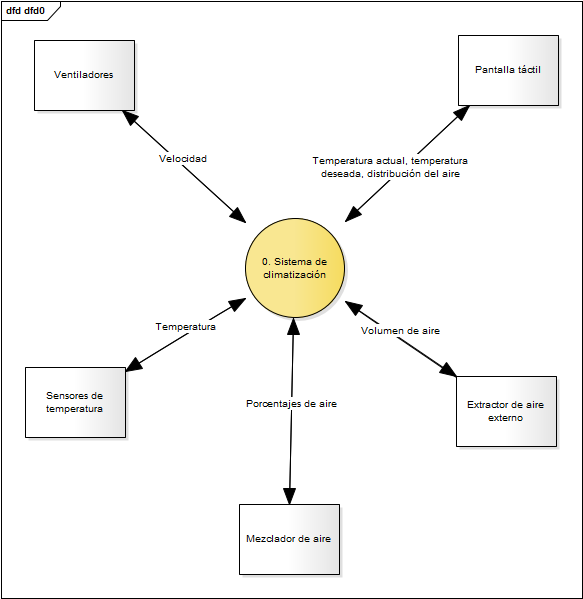
\includegraphics[width=0.8\linewidth]{Resources/dfd0.png}
  \caption{Diagrama de contexto}
  \label{fig:dfd0}
\end{figure}
\begin{figure}[H]
  \centering
  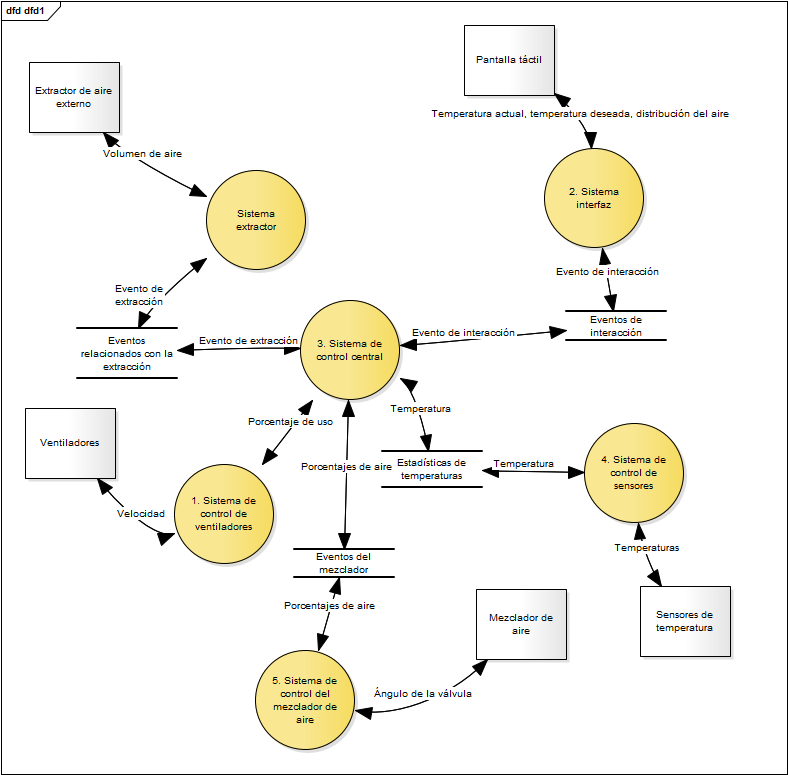
\includegraphics[width=0.8\linewidth]{Resources/dfd1.png}
  \caption{DFD de primer nivel}
  \label{fig:dfd1}
\end{figure}

\subsection{Para la funcionalidad RF1, haz un DFD de nivel 2, con su DFC asociado}


\subsection{En el siguiente contexto ¿cual sería el modelo de ciclo de vida más adecuado? justifica tu respuesta.}
``El software va a ser desarrollado por un empresa de amplia experiencia en el desarrollo de software empotrado, pero nunca para el sector de vivienda familiar. Los requisitos están perfectamente definidos, pero la competencia está muy activa, lo que puede resultar en una modificación de requisitos para adoptarlo a las nuevas funcionalidades. Las pantallas táctiles están empezando a ser comercializadas por lo que no se sabe muy bien como es el paradigma de iteración con el usuario''
%XP o Espiral??

\paragraph{Una posible solución:} El ciclo de vida recomendado es el ``ciclo de vida en espiral''. Los motivos son los siguientes:
\begin{itemize}
\item Los requisitos están bien definidos y los únicos cambios posibles parecen ser la adaptación de nuevas funcionalidades. Como se suceden en varias iteraciones es trivial incorporar esto.
\item No se sabe como es el paradigma de interacción con el usuario por lo que interesa crear prototipos para ello. Este ciclo de vida lo permite (pues en cada iteración hay que tener un producto ejecutable). Además, hay que tener en cuenta que la inexperiencia en el sector familiar refuerza este argumento pues varias iteraciones permiten refinar y mejorar el producto.
\end{itemize}

\subsection{Establece el proceso de admisión de riesgos, según la metodología de Sommerville, que contempla solo 2 riesgos, para el desarrollo de software en el siguiente contexto}
``Vamos a adquirir pantallas táctiles a una empresa china que opera por internet. Tenemos un simulador para el desarrollo de software, que emula el entorno de la vivienda pero no es muy estable, y además no tenemos acceso continuado al prototipo de vivienda en la que se va a verificar y validar el software.

\begin{enumerate}
    \item \textbf{Retraso en la realización de pruebas}
    
    \begin{itemize}
    \item \textbf{Descripción:} Problemas de estabilidad en el software de pruebas o incapacidad para probar el software en un entorno real pueden producir retrasos tanto en el desarrollo normal como en la realización de las pruebas del software.
    \item \textbf{Probabilidad:} Alto.
    \item \textbf{Impacto:} Serio.
    \item \textbf{Tipo de riesgo:} Del Proyecto.
    \item \textbf{Tratamiento:} Minimización.
    \item \textbf{Acción:} Toma de contacto por parte de nuestro equipo con el simulador utilizado antes de las pruebas en si del programa, para conocer que errores da este y no confundirlos con errores del software desarrollado.
    \item \textbf{Secuencia de seguimiento:} Semanal.
    \item \textbf{Indicadores de riesgo:} 
    \begin{itemize}
        \item La realización de pruebas se retrasa durante la fase de utilización de la simulación en las pruebas.
        \item imposibilidad de encontrar un lugar donde hacer la verificación y validación definitivas.
        \item Surgen reportes de fallos del software de simulación durante las pruebas que deberían haberse detectado durante la toma de contacto de nuestro equipo con el software de simulación.
    \end{itemize}
    \end{itemize}

    \item \textbf{Corrupción de todos los archivos del proyecto}
    \begin{itemize}
    \item \textbf{Descripción:} el simulador, debido a su baja estabilidad, corrompe todos los archivos del proyecto.
    \item \textbf{Probabilidad antigua:} Medio.
    \item \textbf{Probabilidad nueva:} Medio.
    \item \textbf{Impacto antiguo:} Catastrófico.
    \item \textbf{Impacto nuevo:} Tolerable.
    \item \textbf{Tipo de riesgo:} Del Producto.
    \item \textbf{Tratamiento:} Minimización.
    \item \textbf{Acción:} Se establecerá un proceso de gestión de la configuración que almacenará en un control de versiones copias diarias de los archivos a utilizar por el simulador.
    \item \textbf{Secuencia de seguimiento:} Diaria.
    \item \textbf{Indicadores de riesgo:}
    \begin{itemize}
        \item Incapacidad de acceder a los archivos del proyecto.
    \end{itemize}
    \end{itemize}
\end{enumerate}


\subsection{Pensando en un proceso de pruebas, establece las clases de equivalencia para las siguientes entradas, asumiendo que en la pantalla táctil se puedan introducir los datos por pantalla con la simulación de un teclado qwerty}
%no entiendo si quiere que todos los datos sean tipo string o algo....
\begin{enumerate}
    \item Temperatura de confort.
    \item Velocidad del ventilador.
    \item Válvula que regula la mezcla aire frío/caliente, asumiendo que la regulación de la misma es por porcentaje, desde 0 (solo aire frío) hasta 100 (solo aire caliente). Cualquier otro valor en el intervalo [0--100] dará una mezcla\%aire\_caliente+\%aire\_frío, de forma que \%aire\_frío=``valor'' y \%aire\_frío=100-``valor''. Este valor no es establecido por teclado, es una variable interna de nuestro software.
\end{enumerate}

%Decimos que es un entero y no un float para no complicar la marrana con los .
\begin{table}[H]
\centering

\resizebox{\textwidth}{!}{%
\begin{tabular}{|c|c|c|c|c|c|c|}
\hline
\multirow{2}{*}{Información} & \multirow{2}{*}{Tipo dato} & \multirow{2}{*}{Regla} & \multicolumn{2}{c|}{Clase válida} & \multicolumn{2}{c|}{Clase no válida} \\ \cline{4-7} 
                             &                            &                        & Id   & Dominio                    & Id         & Dominio                 \\ \hline
Temperatura\_confort         & Entero positivo & 1                      & 1    & {[}10, 45{]}               & 2          & {[}0, 10)               \\ \hline
                             &                            &                        &      &                            & 3          & (45, +inf)              \\ \hline
                             &                            & 3                      & 4    & Está compuesto de dígitos  & 5          & Contiene letras         \\ \hline
\end{tabular}
}
\caption{Clases de equivalencia para ``Temperatura confort''}
\end{table}

%Es la regla 2o la cuatro?
\begin{table}[H]
\centering
\resizebox{\textwidth}{!}{%
\begin{tabular}{|c|c|c|c|c|c|c|}
\hline
\multirow{2}{*}{Información} & \multirow{2}{*}{Tipo dato} & \multirow{2}{*}{Regla} & \multicolumn{2}{c|}{Clase válida} & \multicolumn{2}{c|}{Clase no válida} \\ \cline{4-7} 
                             &                            &                        & Id          & Dominio             & Id           & Dominio               \\ \hline
Velocidad\_ventilador        & Entero positivo            & 2                      & 1           & {[}0, 5{]}          & 2            & (-inf, -1{]}          \\ \hline
                             &                            &                        & 8           & 2                   & 3            & {[}6, +inf)           \\ \hline
                             &                            &                        & 4           & 3                   &              &                       \\ \hline
                             &                            &                        & 5           & 4                   &              &                       \\ \hline
                             &                            &                        & 6           & 5                   &              &                       \\ \hline
                             &                            &                        & 7           & 0                   &              &                       \\ \hline
\end{tabular}
}
\caption{Clases de equivalencia para ``Velocidad del ventilador''}
\end{table}

% Lo hago solo para el valor, que es lo que hay que probar
\begin{table}[h]
\centering
\resizebox{\textwidth}{!}{%
\begin{tabular}{|c|c|c|c|c|c|c|}
\hline
\multirow{2}{*}{Información} & \multirow{2}{*}{Tipo dato} & \multirow{2}{*}{Regla} & \multicolumn{2}{c|}{Clase válida} & \multicolumn{2}{c|}{Clase no válida} \\ \cline{4-7} 
                             &                            &                        & Id         & Dominio              & Id           & Dominio               \\ \hline
Valor\_mezcla                & Punto flotante             & 1                      & 1          & {[}0, 100{]}         & 2            & (-inf, 0)             \\ \hline
                             &                            &                        &            &                      & 3            & (100, +inf)           \\ \hline
\end{tabular}
}
\caption{Clases de equivalencia para el ``valor de la mezcla''}
\end{table}

% \begin{figure}[H]
%   \centering
%   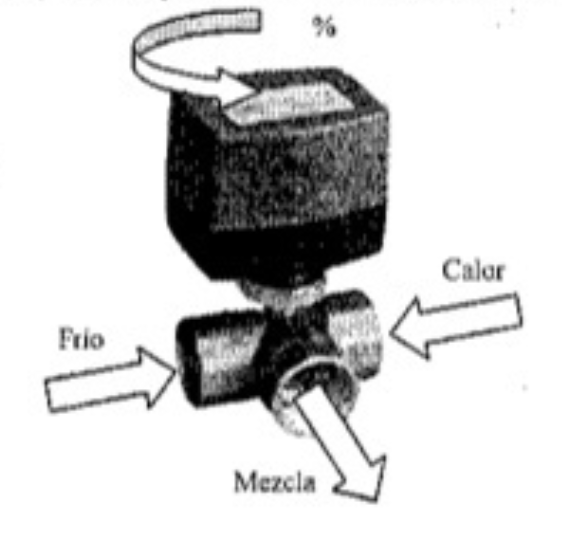
\includegraphics[width=0.5\linewidth]{Resources/imagenExamen2014}
%   \caption{Funcionamiento del aire}
%   \label{fig:aireAcondicionado}
% \end{figure}
